\section{Implementation}

In this section we describe an implementation of the method described in
section \ref{label{sec:method}} suitable for rapid gravitational-wave searches
for compact binary coalescence.  The previous method requires several
computations that can be done before the analysis is actually underway.  Thus
we divide the procedure into two stages 1) an offline planning stage and 2) an
online, low latency filtering stage.  The offline stage can be done before the
analysis is started and updated asychronously, whereas the online stage must keep
up with the detector output and produce search results as rapidly as possible.
In the next two subsections we describe what these stages entail.

\subsection{Planning stage}

The choice of filter waveforms and singular value decomposition can be done in
advance and will be valid as long as the detector noise spectrum remains
roughly constant.  New filter waveforms can be computed asynchronously using
updated spectrum estimates as they are available. 

The planning stage begins with choosing templates that cover the space of mass
parameters with a hexagonal grid \cite{PhysRevD.76.102004} in order to satisfy
the minimum match criterion, which assures a user specified maximum loss in SNR
for signals that fall in-between the chosen templates.  Next, the templates are
subdivided into groups of neighbors called ``sub-banks'' that are appropriately
sized so that each bank can be efficiently handled by a single computer.
Dividing the mass space into smaller sub-banks also aids in the computational
cost of the singular value decomposition and is the approach considered
in~\cite{Cannon:2010p10398}.  Using our understanding of the time-frequency
evolution of the templates, we choose time slice boundaries as in \eqref{FIXME}
such that all of the templates within a sub-bank are sub-critically sampled at
progressively lower sample rates.  Next, the templates within the sub-bank are
realized as \textsc{fir} filter coefficients.  For each time slice, the
templates are downsampled to the appropriate sample rate.  Finally, the
\textsc{svd} is applied to each time slice in the sub-bank in order to produce
a set of orthogonal \textsc{fir} filters and a reconstruction matrix that maps
them back to the original templates as described in \eqref{FIXME}.  The
downsampled orthogonal \textsc{fir} filter coefficients, the reconstruction
matrix, and the time slice boundaries are all saved to disk.

\subsection{Filtering stage}

The filtering algorithm described in the previous section could be used in a
true sample-in-sample-out realtime system.  This would likely require a
nontrivial integration directly into the data acquisition and storage system of
the gravitational wave observatories.  A slightly more modest goal is to leverage
existing low latency, but not realtime, signal processing infrastructure in
order to implement the algorithm described in the previous section.   

We have implemented a prototype of the low latency filtering stage using an
open source signal processing environment called \gstreamer\ \cite{gstreamer}.
\gstreamer\ is a vital component of many Linux systems, providing media
playback, authoring, and streaming on devices from cell phones to desktop
computers to streaming media servers.  Given the similarities of gravitational
wave detector data to audio data it is not surprising that \gstreamer\ is
useful.  In our application, GStreamer excels at queueing, synchronizing,
adding, and bookkeeping many different signals at different sample rates.  It
also provides some useful signal processing elements such as decimators,
\textsc{fir} filters, and interpolators.  

\begin{figure}[htbp]
	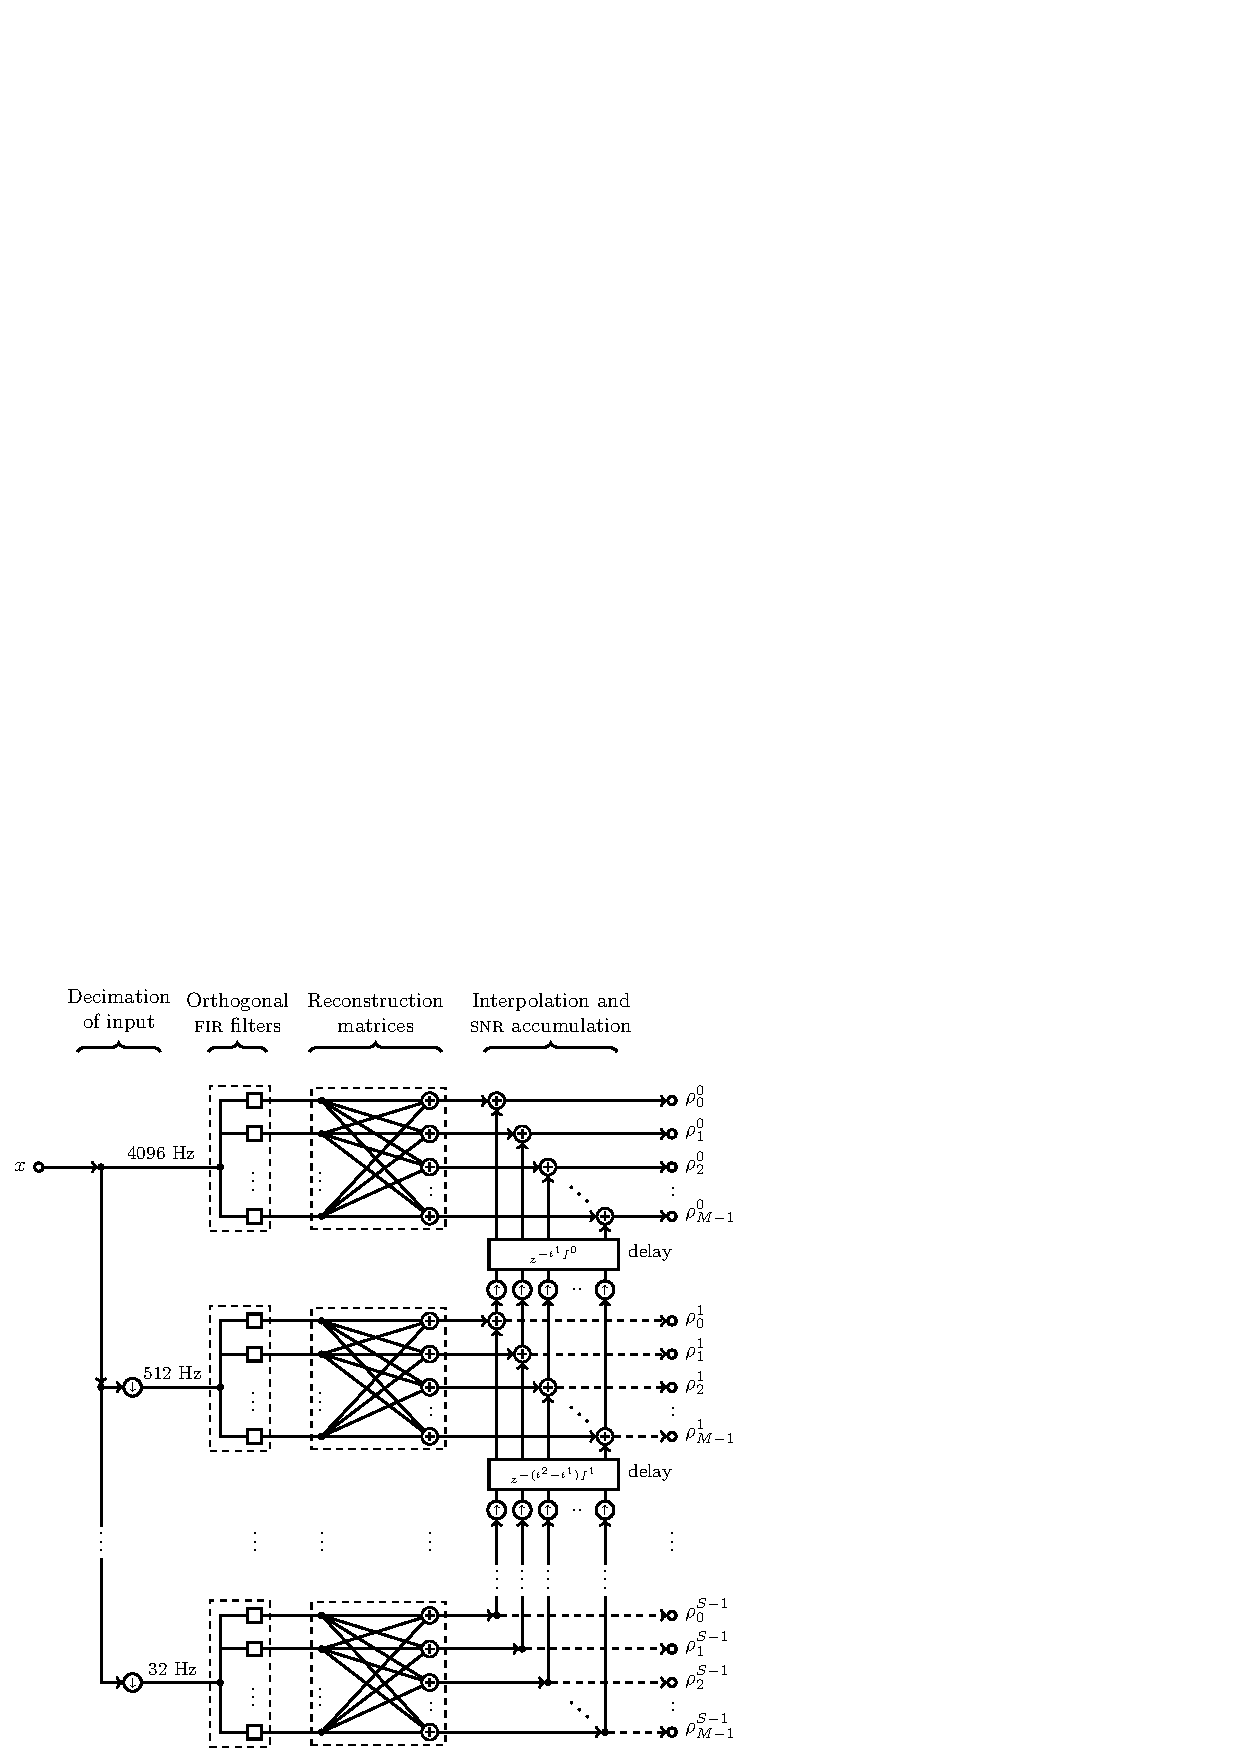
\includegraphics{figures/lloid-diagram.pdf}
	\caption{Schematic of LLOID pipeline illustrating signal flow.  Circles with arrows represent upsampling \protect\includegraphics{figures/upsample-symbol.pdf} or downsampling \protect
\includegraphics{figures/downsample-symbol.pdf}.  Circles with plus signs represent summing junctions \protect\includegraphics{figures/adder-symbol.pdf}.  Squares \protect\includegraphics{figures/fir-symbol.pdf} stand for FIR filters.  Sample rate decreases from the top of the diagram to the bottom.}
\end{figure}

The filter pipeline consists of six distinct stages.  

\subsubsection{Decimation}

First, the sample rate of the whitened detector data is reduced to successively
lower sample rates by decimation.  Decimation involves applying an antialiasing
filter to the data, and then downsampling by deleting samples.  We use a
192-tap \textsc{fir} decimator provided by {\tt Gstreamer's audioresample} element.
The detector data is provided at every power-of-two sample rate required by the 
template time sliced described in \ref{FIXME}. 

\subsubsection{Time delays}

Rather than implement the time sliced templates as zero padded \fir\ filters as
described in \eqref{FIXME} we instead implement them as shorter, but
appropriately time delayed \fir\ filters that contain only the nonzero samples.
In order to assure that we add the \SNR from the time slices adds appropriate


Each decimated detector data stream becomes the input for one time slice, but
it must be appropriately delayed.

\subsubsection{Orthogonal \textsc{fir} filters}

\subsubsection{Reconstruction}

\subsubsection{Interpolation}

\subsubsection{SNR accumulation}
